\section[toc=$\nu N$ interactions]{Neutrino interactions: free nucleon}

\begin{slide}[toc=(Q)EL scattering]{(Quasi-)elastic scattering}
\null\vfill
  
  \twocolumn
  {
    \begin{itemize}
     \item Llewellyn-Smith model is usually used for charged current quasi-elastic scattering
     \item Not much difference here between generators (but default parameters)
    \end{itemize}
  }
  {
    \scalebox{0.75}{\begin{tikzpicture}[node distance = 1cm and 1.5cm]
  
 \node(left) [] {};
 \node(leftEmpty) [left=of left] {};
 \node(leftUp) [above=of leftEmpty] {$\nu / l$};
 \node(leftDown) [below=of leftEmpty] {$\nu$};
 
 \node(right) [right=of left] {};
 \node(rightEmpty) [right=of right] {};
 \node(rightUp) [above=of rightEmpty] {N'};
 \node(rightDown) [below=of rightEmpty] {N};
 
 \draw[curl, thick] (left.center) -- node[above] {$Z^0 / W^\pm$} ++ (right.center);
 
 \draw[color = pdcolor1, thick] (left.center) -- (leftUp);
 \draw[color = pdcolor1, thick] (left.center) -- (leftDown); 
 \draw[color = pdcolor1, thick] (right.center) -- (rightUp);
 \draw[color = pdcolor1, thick] (right.center) -- (rightDown);
 
\end{tikzpicture}
}
  }
  
  \sep
  
  \twocolumn
  {
    \centering\scalebox{0.5}{\begin{tikzpicture}
  
  \node (n) [circle, filled, minimum width = 4cm] {};

  \node (q1) [circle, filled={pdcolor5}, minimum width = 1cm, below=of n, yshift = 4.75cm] {}; 
  \node (q2) [circle, filled={pdcolor6}, minimum width = 1cm, below=of q1, xshift = 1cm] {}; 
  \node (q3) [circle, filled={pdcolor7}, minimum width = 1cm, below=of q1, xshift = -1cm] {};
 
  \draw [curl={pdcolor2}, very thick] (q1) -- (q2);
  \draw [curl={pdcolor2}, very thick] (q2) -- (q3);
  \draw [curl={pdcolor2}, very thick] (q3) -- (q1);

\end{tikzpicture}
}
  }
  {
    \sep
    \begin{itemize}
     \item Nucleon structure is parametrized by form factors
    \end{itemize}
  }

  \begin{itemize}
    \item Vector $\rightarrow$ Conserved Vector Current (CVC)
    \item Pseudo-scalar $\rightarrow$ Partially Conserved Axial Current (PCAC)
    \item Axial $\rightarrow$ dipole form with one free parameter (axial mass, $M_A$)
  \end{itemize}

  
\vfill\null
\end{slide}

\begin{wideslide}{Rein-Sehgal model}
\null\vfill

  \twocolumn
  {
    \sep\sep\sep
 
    \centering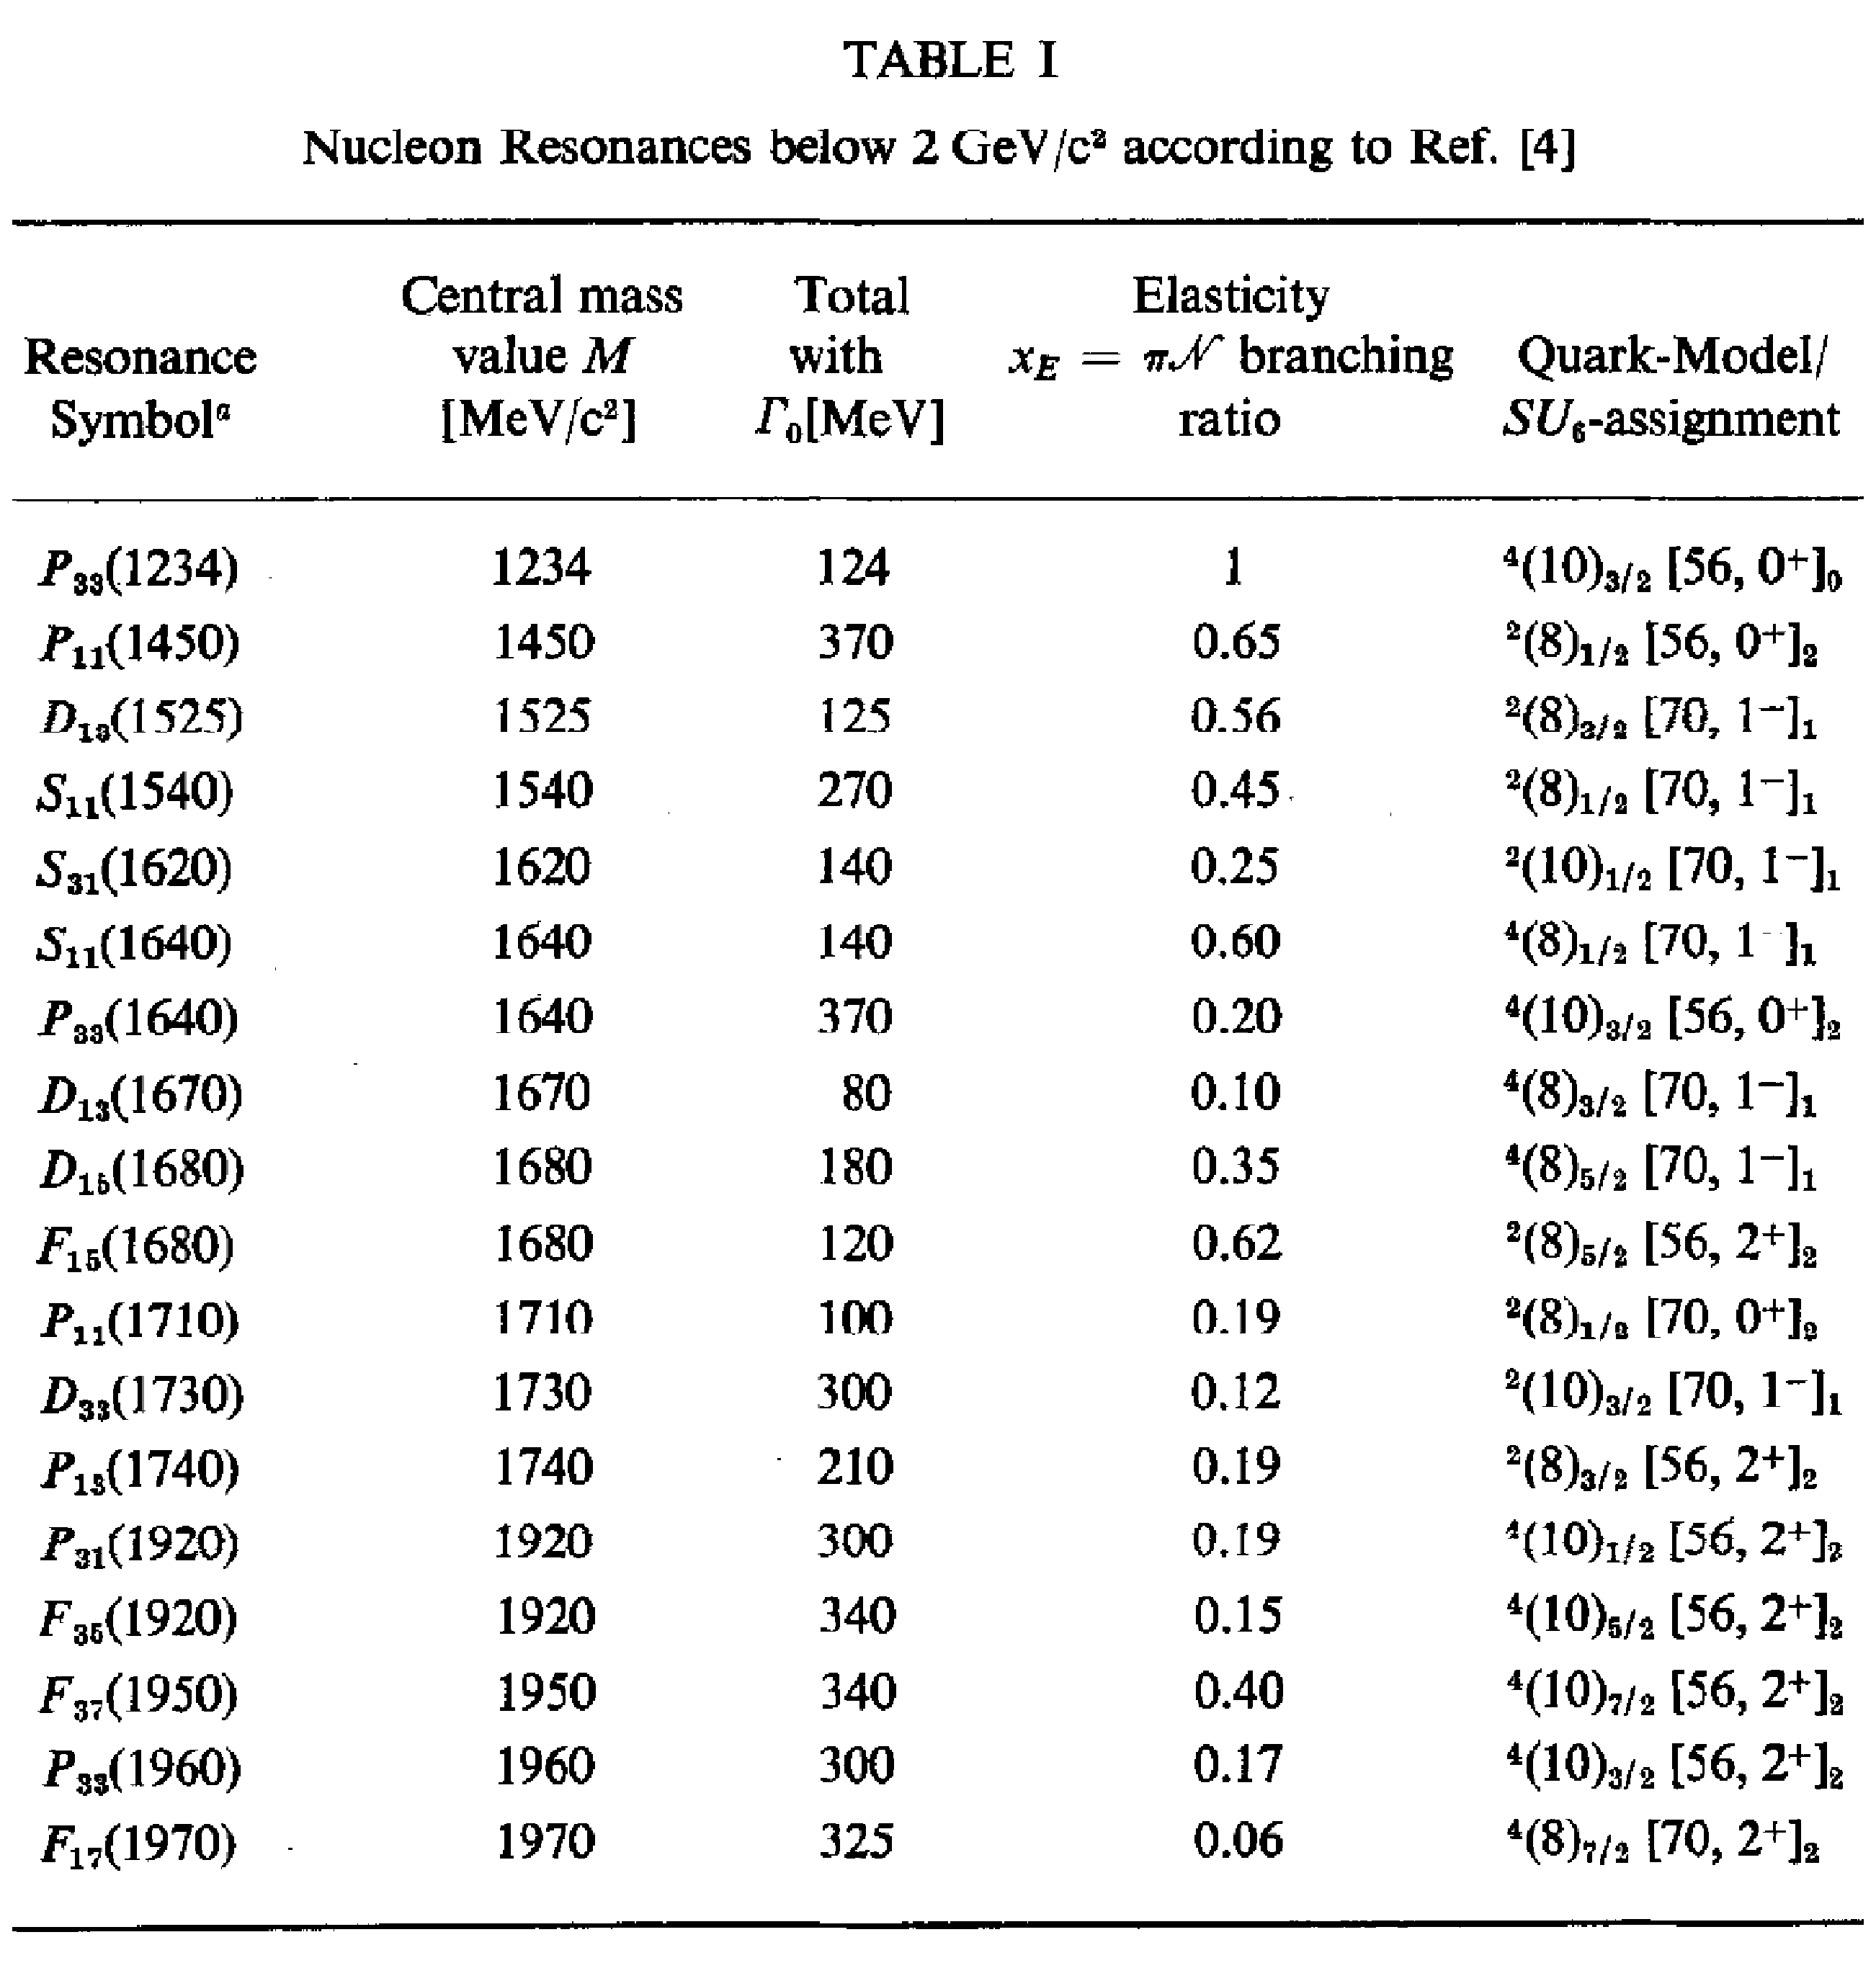
\includegraphics[width=\columnwidth]{figures/rein.eps}
  }
  {
    \centering\begin{tikzpicture}[node distance = 1cm and 1.5cm]
  
 \node(left) [] {};
 \node(leftEmpty) [left=of left] {};
 \node(leftUp) [above=of leftEmpty] {$\nu / l$};
 \node(leftDown) [below=of leftEmpty] {$\nu$};
 
 \node(right) [right=of left] {};
 \node(rightEmpty) [right=of right] {};
 \node(rightDown) [below=of rightEmpty] {N};

 \node(delta) [above=of rightEmpty, xshift = -1.0cm, yshift = -0.5cm] {$\Delta$};
 \node(rightUp1) [above=of delta, yshift = -0.5cm] {$\pi$};
 \node(rightUp2) [right=of delta, xshift = -1.0cm] {N'};
 
 \draw[curl, thick] (left.center) -- node[above] {$Z^0 / W^\pm$} ++ (right.center);
 
 \draw[color = pdcolor1, thick] (left.center) -- (leftUp);
 \draw[color = pdcolor1, thick] (left.center) -- (leftDown); 
 \draw[color = pdcolor1, thick] (right.center) -- (rightDown);
 \draw[color = pdcolor1, thick] (right.center) -- (delta);
 \draw[color = pdcolor1, thick] (delta) -- (rightUp1);
 \draw[color = pdcolor1, thick] (delta) -- (rightUp2);
 
\end{tikzpicture}

    \begin{itemize}
     \item Rein-Sehgal model describes single pion production through baryon resonances below $W = 2$~GeV
     \item It is used by GENIE and NEUT
     \item However, GENIE includes only 16 resonances and interference between them is neglected
    \end{itemize}
  }	

\vfill\null
\end{wideslide}

\begin{slide}[toc=Deep Inelastic Scattering]{Deep inelastic scattering [DIS]}
\null\vfill

  \twocolumn
  {
    \sep
    \begin{itemize}
     \item Quark-parton model is used for deep inelastic scattering
     \item Bodek-Young modification to the parton distributions at low $Q^2$ is included by most generators
    \end{itemize}
  }
  {
    \scalebox{0.75}{\begin{tikzpicture}[node distance = 1cm and 1.5cm]
  
 \node(left) [] {};
 \node(leftEmpty) [left=of left] {};
 \node(leftUp) [above=of leftEmpty] {$\nu / l$};
 \node(leftDown) [below=of leftEmpty] {$\nu$};
 
 \node(right) [right=of left] {};
 \node(rightEmpty) [right=of right] {};
 \node(rightDown) [below=of rightEmpty, xshift = -0.2cm, yshift = 0.2cm] {\scalebox{0.2}{\begin{tikzpicture}
  
  \node (n) [circle, filled, minimum width = 4cm] {};

  \node (q1) [circle, filled={pdcolor5}, minimum width = 1cm, below=of n, yshift = 4.75cm] {}; 
  \node (q2) [circle, filled={pdcolor6}, minimum width = 1cm, below=of q1, xshift = 1cm] {}; 
  \node (q3) [circle, filled={pdcolor7}, minimum width = 1cm, below=of q1, xshift = -1cm] {};
 
  \draw [curl={pdcolor2}, very thick] (q1) -- (q2);
  \draw [curl={pdcolor2}, very thick] (q2) -- (q3);
  \draw [curl={pdcolor2}, very thick] (q3) -- (q1);

\end{tikzpicture}
}};

 \node(rightUp) [above=of rightEmpty, xshift = -0.2cm, yshift = 0.2cm] {\scalebox{0.2}{\begin{tikzpicture}
  
  \node (center) {};
  
  \node [circle, filled={pdcolor4}, minimum width = 1cm, below=of center, xshift = 3cm, yshift = 0cm] {}; 
  \node [circle, filled={pdcolor5}, minimum width = 1cm, below=of center, xshift = 6cm, yshift = 1cm] {}; 
  \node [circle, filled={pdcolor6}, minimum width = 1cm, below=of center, xshift = 2cm, yshift = 2cm] {}; 
  \node [circle, filled={pdcolor7}, minimum width = 1cm, below=of center, xshift = 0cm, yshift = 3cm] {}; 
  \node [circle, filled={pdcolor4}, minimum width = 1cm, below=of center, xshift = 1cm, yshift = 4cm] {}; 
  \node [circle, filled={pdcolor5}, minimum width = 1cm, below=of center, xshift = 4cm, yshift = 3.5cm] {}; 
  \node [circle, filled={pdcolor6}, minimum width = 1cm, below=of center, xshift = 2.5cm, yshift = 3.5cm] {}; 
  \node [circle, filled={pdcolor7}, minimum width = 1cm, below=of center, xshift = 4.25cm, yshift = 1.5cm] {}; 
 
\end{tikzpicture}
}};
 
 \draw[curl, thick] (left.center) -- node[above] {$Z^0 / W^\pm$} ++ (right.center);
 
 \draw[color = pdcolor1, thick] (left.center) -- (leftUp);
 \draw[color = pdcolor1, thick] (left.center) -- (leftDown); 
 \draw[color = pdcolor1, thick, shorten >= -10pt] (right.center) -- (rightDown);

 \draw[color = pdcolor1, thick, shorten >= -10pt] (right.center) -- (rightUp);

\end{tikzpicture}
}
  }
  
  \myBoxFullWidth{Hadronization}
  
  \twocolumn
  {
    \sep\sep\sep
    \centering\scalebox{0.75}{\begin{tikzpicture}[node distance = 2cm]
  
  \node (quarks) {\scalebox{0.2}{\begin{tikzpicture}
  
  \node (center) {};
  
  \node [circle, filled={pdcolor4}, minimum width = 1cm, below=of center, xshift = 3cm, yshift = 0cm] {}; 
  \node [circle, filled={pdcolor5}, minimum width = 1cm, below=of center, xshift = 6cm, yshift = 1cm] {}; 
  \node [circle, filled={pdcolor6}, minimum width = 1cm, below=of center, xshift = 2cm, yshift = 2cm] {}; 
  \node [circle, filled={pdcolor7}, minimum width = 1cm, below=of center, xshift = 0cm, yshift = 3cm] {}; 
  \node [circle, filled={pdcolor4}, minimum width = 1cm, below=of center, xshift = 1cm, yshift = 4cm] {}; 
  \node [circle, filled={pdcolor5}, minimum width = 1cm, below=of center, xshift = 4cm, yshift = 3.5cm] {}; 
  \node [circle, filled={pdcolor6}, minimum width = 1cm, below=of center, xshift = 2.5cm, yshift = 3.5cm] {}; 
  \node [circle, filled={pdcolor7}, minimum width = 1cm, below=of center, xshift = 4.25cm, yshift = 1.5cm] {}; 
 
\end{tikzpicture}
}};
  \node (hadrons) [ell, notFilled, right=of quarks] {Hadrons};
  
  \draw [line, ->] (quarks) -- (hadrons);
 
\end{tikzpicture}
}
  }
  {
    \begin{itemize}
     \item Hadronization is the process of formation hadrons from quarks
     \item Pythia is widely used at high invariant masses
    \end{itemize}
  }

\vfill\null
\end{slide}

\begin{slide}[toc=AGKY model]{Andreopoulos-Gallagher-Kehayias-Yang model}
\null\vfill

  \sep

  \twocolumn
  {
    \begin{itemize}
     \item AGKY hadronization model is used in GENIE
    \end{itemize}
  }
  {
    \centering\scalebox{0.75}{\begin{tikzpicture}[node distance = 2cm]
  
  \node (quarks) {\scalebox{0.2}{\begin{tikzpicture}
  
  \node (center) {};
  
  \node [circle, filled={pdcolor4}, minimum width = 1cm, below=of center, xshift = 3cm, yshift = 0cm] {}; 
  \node [circle, filled={pdcolor5}, minimum width = 1cm, below=of center, xshift = 6cm, yshift = 1cm] {}; 
  \node [circle, filled={pdcolor6}, minimum width = 1cm, below=of center, xshift = 2cm, yshift = 2cm] {}; 
  \node [circle, filled={pdcolor7}, minimum width = 1cm, below=of center, xshift = 0cm, yshift = 3cm] {}; 
  \node [circle, filled={pdcolor4}, minimum width = 1cm, below=of center, xshift = 1cm, yshift = 4cm] {}; 
  \node [circle, filled={pdcolor5}, minimum width = 1cm, below=of center, xshift = 4cm, yshift = 3.5cm] {}; 
  \node [circle, filled={pdcolor6}, minimum width = 1cm, below=of center, xshift = 2.5cm, yshift = 3.5cm] {}; 
  \node [circle, filled={pdcolor7}, minimum width = 1cm, below=of center, xshift = 4.25cm, yshift = 1.5cm] {}; 
 
\end{tikzpicture}
}};
  \node (hadrons) [ell, notFilled, right=of quarks] {Hadrons};
  
  \draw [line, ->] (quarks) -- (hadrons);
 
\end{tikzpicture}
}  
  }
  
  \begin{itemize}
    \item It includes phenomenological description of the low invariant mass based on Koba-Nielsen-Olesen (KNO) scaling
    \item Pythia is used for the high invariant mass
    \item The smooth transition between two models is made in a window $W \in [2.3, 3.0]$~GeV
  \end{itemize}
  
  \sep
  
  \centering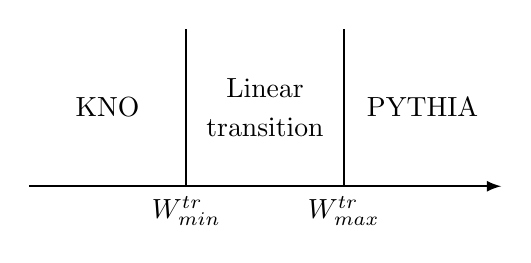
\begin{tikzpicture}
  
  \draw[>=latex, ->, thick] (0, 0) -- (6,0);
  
  \draw[thick] (2,0) -- node[below] {$W^{tr}_{min}$} (2,0) -- (2,2);
  \draw[thick] (4,0) -- node[below] {$W^{tr}_{max}$} (4,0) -- (4,2);
  
  \node at (1,1) {KNO};
  \node at (5,1) {PYTHIA};
  \node at (3,1.25) {Linear};
  \node at (3,0.75) {transition};
  
\end{tikzpicture}


\vfill\null
\end{slide}

\begin{slide}[toc=$\pi$ in NuWro]{Pion production in NuWro}
\null\vfill

  \centering\begin{tikzpicture}[node distance = 1.5cm and 1cm]
 
 \node(empty) {};
 
 \node(piprod) [rect, round, filled, above=of empty] {$\pi$ production};
 \node(delta)  [rect, notFilled, left=of empty, align = center] {$\Delta$ resonance \\ {\tiny Adler-Rarita-Schwinger}};
 \node(quark)  [rect, notFilled, right=of empty] {Quark-parton model};
 
 \node(res) [ell, filled, below=of delta] {RES};
 \node(dis) [ell, filled, below=of quark] {DIS};
 
 \draw [line, thick, ->] (piprod) -- (delta);
 \draw [line, thick, ->] (piprod) -- (quark);
 \draw [line, thick, ->] (delta) -- (res);

 \draw [line, thick, ->] (quark) -- node[above, rotate=25] {$W < 1.6$ GeV} ++ (res);
 \draw [line, thick, ->] (quark) -- node[right] {$W > 1.6$ GeV} ++ (dis);

 
\end{tikzpicture}


  \sep\sep
  
  \myFrameTextWidth[pdcolor6]{RES/DIS distinguish is arbitrary for each MC generator!}

\vfill\null
\end{slide}

\begin{wideslide}{Transition region}
\null\vfill

  \begin{itemize}
    \item We factorized the reality to RES and DIS 
    \item We must be careful to avoid double counting
    \item The smooth transition between RES and DIS is performed by each generator (but in slightly different way)
    \item E.g. in GENIE:
  \end{itemize}
    
  \begin{eqnarray*}
    \frac{d^2\sigma^{RES}}{dQ^2dW} & = & \sum\limits_k \left(\frac{d^2\sigma^{R-S}}{dQ^2dW}\right)_k\cdot\Theta(W_{cut} - W) \\
    \frac{d^2\sigma^{DIS}}{dQ^2dW} & = & \frac{d^2\sigma^{DIS,BY}}{dQ^2dW}\cdot\Theta(W - W_{cut}) + \frac{d^2\sigma^{DIS,BY}}{dQ^2dW}\cdot\Theta(W_{cut} - W)\cdot\sum\limits_m f_m
  \end{eqnarray*}
  
  \sep
  
  where $k$ - sum over resonances in Rein-Sehgal model, $m$ - sum over multiplicity, $f_m = R_m\cdot P_m$ with $P_m$ - probability of given multiplicity (taken form hadronization model), $R_m$ - tunable parameter

\vfill\null
\end{wideslide}